\begin{figure}[tp]
\centering
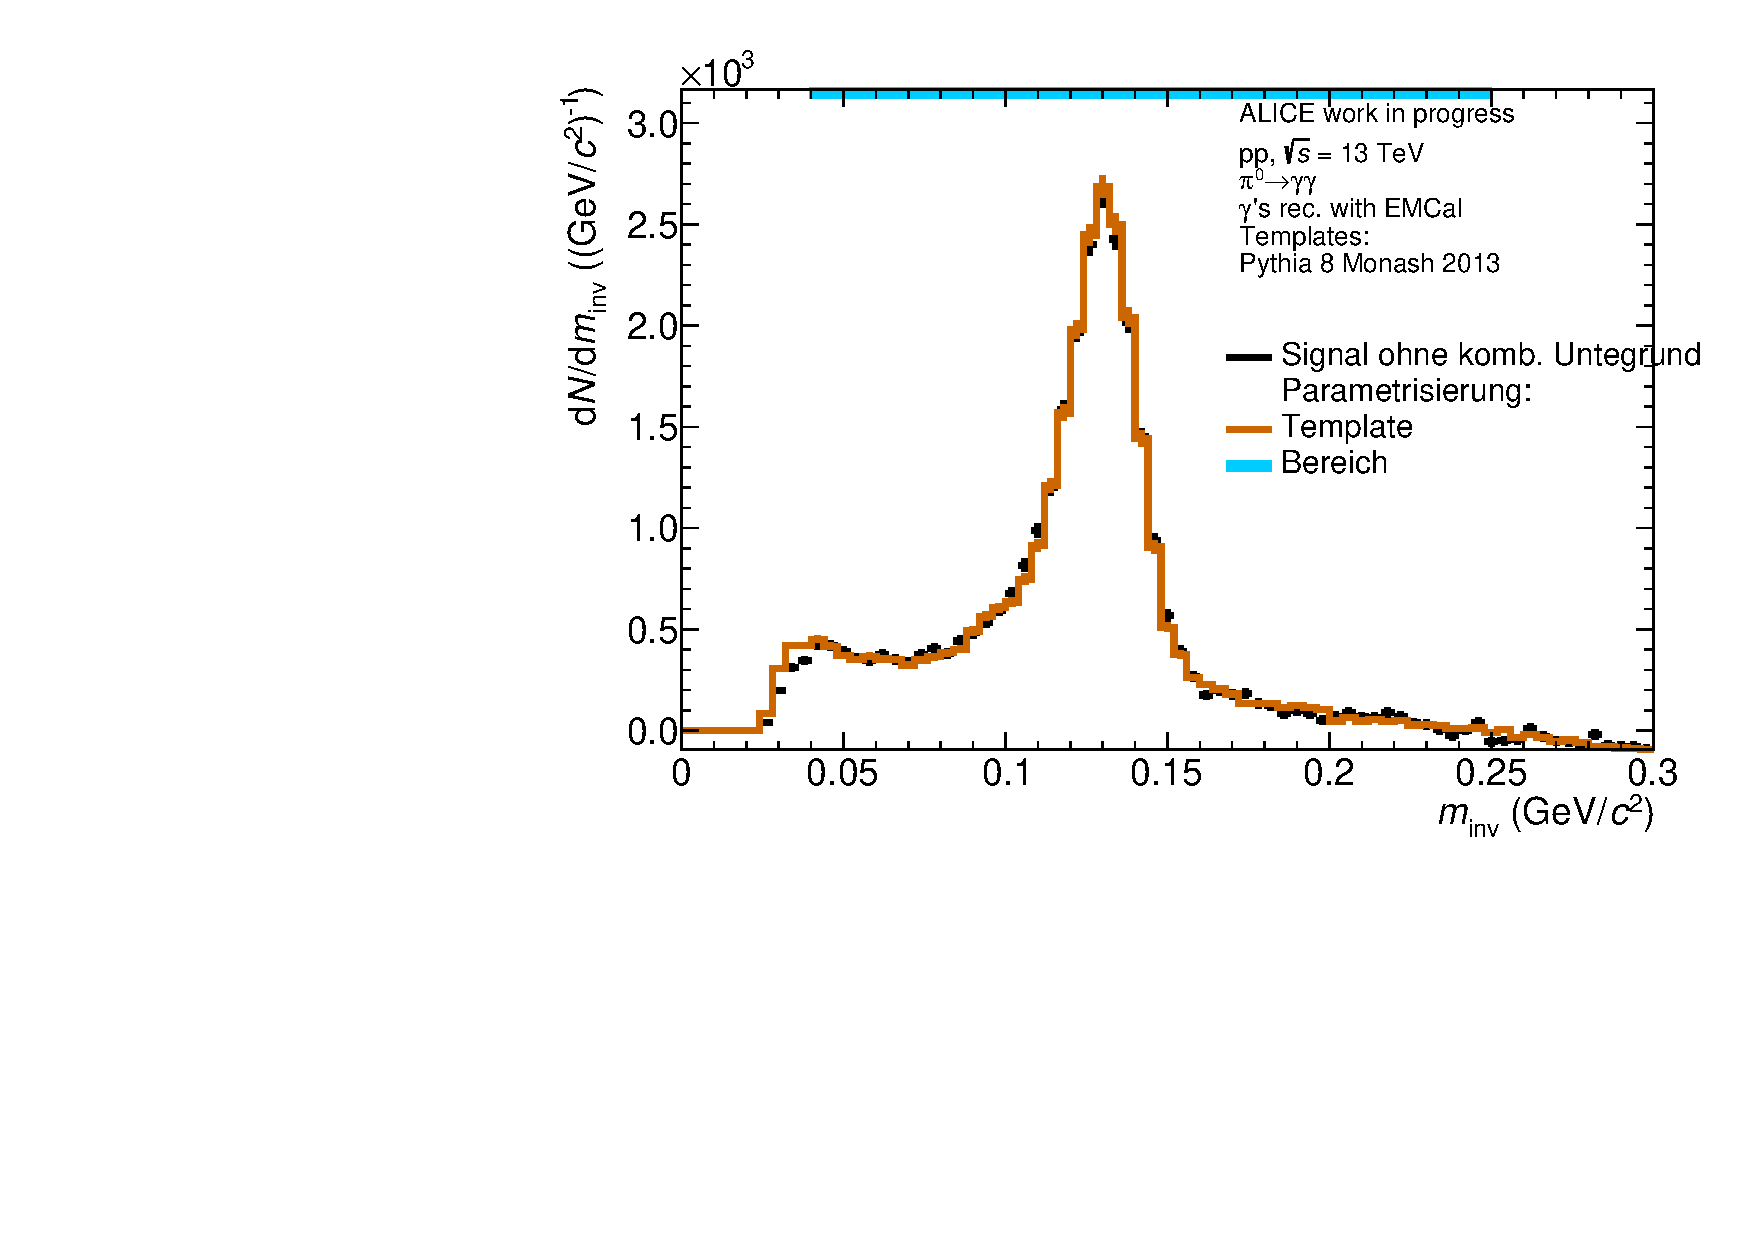
\includegraphics[width=.65\linewidth]{ParamResult_Bin10_Data_2016.pdf}
\caption{Signal mit unkorreliertem Untergrund zusammen mit Parametrisierung der Templates des korrelierten Untergrund und des Signals.
}
\label{fig:ParamResult}
\end{figure}
Das Ergebnis der Parametrisierung der Templates für das $p_\text{T}$-Intervall $(3\,2-3\,4)(\text{GeV/}c)$ wird in Abbildung \ref{fig:ParamResult} dargestellt.
Die Parametrisierung der beiden Templates stimmt innerhalb der Unsicherheiten gut mit den Daten überein, wie zu erwarten war, nach Abbildung \ref{fig:Chi2pT}.
%%detaillierter Beschreiben was man sieht?????
\newline
Um die Anzahl produzierter $\pi^{0}$ nun zu bestimmen, wird das skalierte Template des korrelierten Untergrunds von dem Signal ohne kombinatorischen Untergrund abgezogen.
Anschließend wird in einem bestimmten Zählbereich über die Werte des Signals summiert.
Dies wird für jedes $p_\text{T}$-Intervall durchgeführt.
\newline
Der Zählbereich hängt dabei von $p_\text{T}$ ab, da er so gewählt wurde, dass die untere Grenze immer groß genug ist, um nicht von den Anforderungen an den Öffnungswinkel betroffen zu sein.
Die obere Grenze liegt fest bei $p_\text{T} = 0\,25 \text{ GeV}/c$.
In Abbildung \ref{fig:ParamResult} wird er Zählbereich durch eine blaue Linie markiert.
\begin{figure}[tp]
\centering
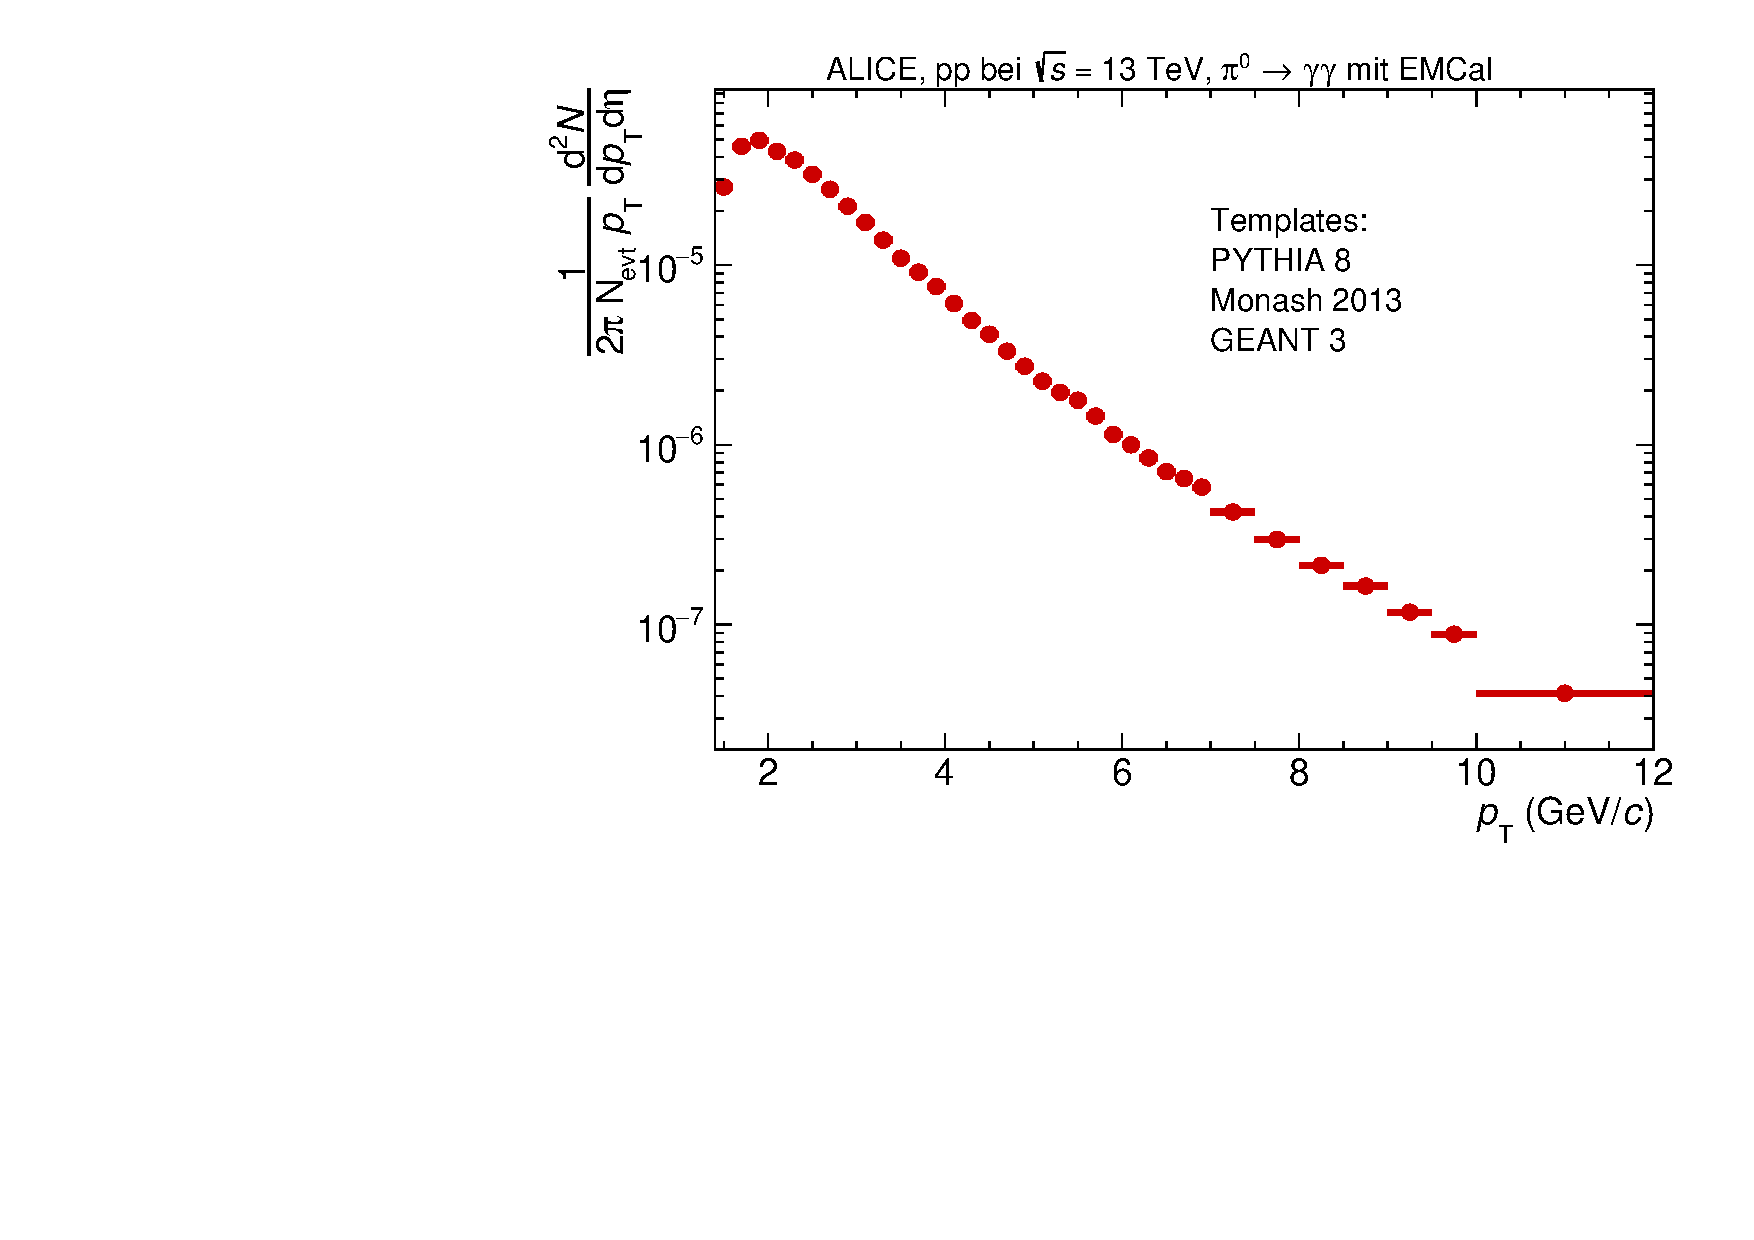
\includegraphics[width=.65\linewidth]{UncorrYields_Data_2016.pdf}
\caption{Anzahl produzierter $\pi^{0}$ in Abhängigkeit von $p_\text{T}$.
}
\label{fig:RawYield}
\end{figure}
\newline
Das so erhaltene rohe Spektrum wird zusätzlich noch normiert, auf die Anzahl an \textit{events} $N_\text{evt}$, den Pseudorapiditätsbereich $\eta$, den Transversalimpuls $p_\text{T}$, die Wahrscheinlichkeit, dass ein $\pi^{0}$ in zwei Photonen zerfällt und $2\pi$.
Letzteres ist reine Konvention, während die anderen Normierungen einen Vergleich zwischen unterschiedlichen Analysen ermöglichen.
Abbildung \ref{fig:RawYield} zeigt eine normiertes rohes Spektrum.
Das Spektrum steigt zunächst leicht an, bis es bei $1\,8 \leq p_{\text{T}}/(\text{ GeV}/c) < 2\,0$ sein Maximum erreicht.
Danach sinkt das Spektrum kontinuierlich.
\newline
Für eine genaue Aussage über die Produktionsrate von $\pi^{0}$ sowie einen allgemeinen Vergleich wird allerdings noch die Korrektur auf die Detektorakzeptanz sowie die Effizienz benötigt.